\documentclass[12pt,a4paper,oneside]{report}

\usepackage[margin=1in]{geometry}
\usepackage[T1]{fontenc}
\usepackage[utf8]{inputenc}
\usepackage{lmodern}
\usepackage{microtype}
\usepackage{booktabs}
\usepackage{array}
\usepackage{longtable}
\usepackage{tabularx}
\usepackage{multirow}
\usepackage{enumitem}
\usepackage[table]{xcolor}
\usepackage{xurl}
\usepackage{hyperref}
\usepackage{listings}
\usepackage{amsmath}
\usepackage{amssymb}
\usepackage{graphicx}
\usepackage{float}
\usepackage{placeins}
\usepackage{needspace}
\usepackage[font=small,labelfont=bf]{caption}
\usepackage{subcaption}

\hypersetup{
  colorlinks=true,
  linkcolor=blue!45!black,
  citecolor=blue!45!black,
  urlcolor=blue!45!black,
  pdftitle={Graph-Based Machine Learning Pipelines and Automatic Loop Parallelization in Accelera},
  pdfauthor={Mohamed Ashraf}
}

\setlength{\parindent}{0.18in}
\setlength{\parskip}{0.15em}

\lstdefinestyle{paperpython}{
  basicstyle=\ttfamily\footnotesize,
  breaklines=true,
  frame=single,
  columns=fullflexible,
  keepspaces=true,
  showstringspaces=false,
  keywordstyle=\color{blue!55!black},
  commentstyle=\color{green!35!black}
}
\lstdefinestyle{algostyle}{
  basicstyle=\rmfamily\scriptsize,
  backgroundcolor=\color{white},
  frame=tb,
  rulecolor=\color{black},
  framerule=0.45pt,
  framesep=3pt,
  xleftmargin=0pt,
  xrightmargin=0pt,
  numbers=left,
  numberstyle=\scriptsize\rmfamily,
  numbersep=5pt,
  columns=fullflexible,
  keepspaces=true,
  showstringspaces=false,
  breaklines=true,
  breakatwhitespace=false,
  breakautoindent=false,
  breakindent=0pt,
  captionpos=t,
  aboveskip=0.8em,
  belowskip=0.8em
}
\lstset{style=paperpython}
\renewcommand{\lstlistingname}{Algorithm}
\renewcommand{\lstlistlistingname}{List of Algorithms}
\renewcommand{\thelstnumber}{\arabic{lstnumber}:}

\newcommand{\systemname}{Accelera}
\newcommand{\modulepath}[1]{\texttt{#1}}
\newcommand{\todoitem}[1]{\textcolor{red!65!black}{[TODO: #1]}}
\newcommand{\besttime}{\cellcolor{green!20}}
\newcommand{\bestmem}{\cellcolor{blue!15}}

\begin{document}

\begin{titlepage}
\thispagestyle{empty}
\begin{center}

% Cairo University logo and affiliation, adapted from gp_book.tex

\includegraphics[width=0.12\textwidth]{../imgs/CU_logo.png}\\
{\fontsize{12}{14}\selectfont Cairo University}\\
{\fontsize{12}{14}\selectfont Faculty of Engineering}\\
{\fontsize{12}{14}\selectfont Department of Computer Engineering}\\

\vspace{0.9cm}

{\bfseries\fontsize{22}{26}\selectfont Graph-Based Machine Learning Pipelines and Automatic Loop Parallelization in Accelera}

\vspace{0.35cm}

{\fontsize{16}{20}\selectfont Accelera Pipe and Parallelizer Modules}

\vspace{0.9cm}


\includegraphics[width=0.22\textwidth]{../imgs/accelera.png}

\vspace{0.7cm}

{\fontsize{12}{14}\selectfont
A Graduation Project Individual Report Submitted\\
to\\[0.15cm]
Faculty of Engineering, Cairo University\\[0.15cm]
in Partial Fulfillment of the Requirements for the Degree\\[0.15cm]
of\\[0.15cm]
Bachelor of Science in Computer Engineering.
}

\vspace{0.95cm}

{\bfseries\fontsize{16}{18}\selectfont Presented by}

\vspace{0.25cm}

{\fontsize{14}{16}\selectfont Mohamed Ashraf}\\[0.15cm]
{\fontsize{12}{14}\selectfont ID: 9220658}

\vspace{0.75cm}

{\bfseries\fontsize{16}{18}\selectfont Supervised by}

\vspace{0.25cm}

{\fontsize{14}{16}\selectfont Dr. Salma Abdel Monem}

\vspace{0.45cm}

{\fontsize{12}{14}\selectfont June 2026}

\vfill

{\fontsize{11}{14}\selectfont
All rights reserved. This report may not be reproduced in whole or in part,
by photocopying or other means, without the permission of the author or department.
}

\end{center}
\end{titlepage}

\begin{abstract}
This paper describes two core modules of Accelera: \texttt{accelera\_pipe}, a graph-based machine learning pipeline executor, and the Parallelizer, a source-to-source loop optimization module that emits OpenMP-enabled C++ for supported code patterns. The pipeline module represents preprocessing, model fitting, prediction, metrics, branching, merging, and executed inference graphs as a native backend graph. This representation enables parallel branch execution, path selection, graph reuse, and targeted memory optimizations. The Parallelizer converts supported Python code to C++, extracts loops, classifies safe OpenMP transformations, inserts pragmas, and can compile custom preprocessing functions into Python-callable native extensions. Experiments show that \texttt{accelera\_pipe} preserves sklearn-equivalent accuracy while reducing latency on a large four-candidate model-selection benchmark from about 803 seconds to 495 seconds. The Parallelizer also accelerates hard loop examples and reduces a preprocessing-heavy Python kernel from 6.83 seconds to 0.08 seconds in a repeated cached end-to-end pipeline run.\end{abstract}

\tableofcontents
\listoffigures
\listoftables
\clearpage

% -----------------------------------------------------------------------------
\chapter{Introduction}
\label{chap:introduction}
Modern machine learning workflows often require repeated evaluation of several preprocessing and model candidates. A direct implementation usually fits each candidate pipeline independently, repeats transformations, and retains intermediate arrays longer than necessary. In parallel, user-defined preprocessing functions may contain numeric loops written in Python, which can become a major bottleneck when the input data grows.

The project can be viewed as solving two connected execution problems:

\begin{itemize}[leftmargin=1.2cm]
  \item \textbf{Workflow-level inefficiency:} repeated preprocessing, duplicated
  branch execution, and unclear intermediate-data lifetime.
  \item \textbf{Code-level inefficiency:} slow custom Python preprocessing loops
  that could benefit from native compilation and OpenMP parallel execution.
\end{itemize}

Table~\ref{tab:intro-module-scope} summarizes the main scope of the modules
covered by this paper.

\begin{table}[!htbp]
\centering
\caption{Main module scope in this report.}
\label{tab:intro-module-scope}
\small
\renewcommand{\arraystretch}{1.15}
\setlength{\tabcolsep}{4pt}
\begin{tabularx}{\textwidth}{p{0.25\textwidth}X X}
\toprule
Module & Main idea & Expected benefit \\
\midrule
\texttt{accelera\_pipe} &
Represent machine-learning workflows as a graph of preprocessing, model,
prediction, metric, merge, and branch nodes. &
Avoids purely sequential workflow execution and supports reusable executed
graphs. \\

Parallelizer &
Analyze supported Python/C++ loops, insert safe OpenMP pragmas, and compile
optimized native functions when possible. &
Speeds up eligible loop-heavy custom preprocessing code while keeping fallback
behavior safe. \\

Integration path &
Connect the Parallelizer to \texttt{accelera\_pipe} preprocessing nodes. &
Allows pipeline-level execution and code-level acceleration to work together. \\
\bottomrule
\end{tabularx}
\renewcommand{\arraystretch}{1.0}
\end{table}

Accelera addresses these two issues through two complementary modules. The first module, \texttt{accelera\_pipe}, expresses machine learning workflows as a graph. Nodes represent preprocessing steps, models, predictions, metrics, merges, and branch alternatives. The graph backend executes independent branches in parallel and returns an executed graph that can be reused for inference.

The second module, the Parallelizer, analyzes loop-heavy source code and adds OpenMP pragmas when the loop structure is considered safe. For supported Python functions, a restricted Python-to-C++ converter emits C++ code before loop extraction. The generated code can then be compiled into a Python extension and inserted into an \texttt{accelera\_pipe} preprocessing node.

This paper focuses only on these two modules. The main contributions described here are: a graph-based pipeline execution model, memory and branching optimizations for pipeline search, a hybrid rule and classifier loop-parallelization strategy, a documented Python-to-C++ subset, and an integration path that uses the Parallelizer as an acceleration backend for custom preprocessing functions.

% -----------------------------------------------------------------------------
\chapter{Literature Survey}
\label{chap:literature-review}

This chapter reviews the main background and previous work related to the
\systemname{} project. The chapter is divided into four main parts. First, it
introduces machine learning pipeline frameworks, with special attention to
\texttt{scikit-learn}, which is the main practical baseline for the
\texttt{accelera\_pipe} module. Second, it explains the background of automatic
code parallelization and OpenMP, which are needed to understand the design of the
Parallelizer module. Third, it compares the project with related work, especially
\texttt{scikit-learn} pipelines and OMPar, an AI-driven OpenMP parallelization
system. Finally, it explains the implemented approach adopted in this project and
justifies the main design choices, including the use of rule-based pragma
generation instead of fully AI-generated pragma insertion.

The chapter organization is summarized in Table~\ref{tab:literature-map}.

\begin{table}[!htbp]
\centering
\caption{Literature-survey organization.}
\label{tab:literature-map}
\small
\renewcommand{\arraystretch}{1.12}
\setlength{\tabcolsep}{4pt}
\begin{tabularx}{\textwidth}{p{0.30\textwidth}X}
\toprule
Part & Purpose \\
\midrule
Machine-learning pipeline frameworks &
Explains why pipeline abstractions are useful and why
\texttt{scikit-learn} is the main baseline for \texttt{accelera\_pipe}. \\

Automatic parallelization and OpenMP &
Introduces loop-level parallelization, dependency safety, reductions, and
OpenMP pragmas. \\

Comparative study &
Compares Accelera with \texttt{scikit-learn} and OMPar, focusing on what is
borrowed and what is changed. \\

Implemented approach &
Explains why the project combines graph execution with conservative rule-based
OpenMP generation. \\
\bottomrule
\end{tabularx}
\renewcommand{\arraystretch}{1.0}
\end{table}

\section{Background on Machine Learning Pipeline Frameworks}

Machine learning projects rarely consist of a single model call. A complete
workflow usually includes data loading, preprocessing, feature transformation,
model fitting, prediction, metric evaluation, and sometimes several alternative
branches that compare different preprocessing or model choices. Without a
structured pipeline abstraction, these steps can become hard to reproduce and
maintain. For example, preprocessing may accidentally be applied differently
during training and testing, or several experimental branches may repeat the same
early computation many times.

A common Python solution for this problem is the pipeline abstraction provided by
\texttt{scikit-learn}~\cite{pedregosa2011scikit}. In \texttt{scikit-learn}, a
pipeline connects a sequence of transformers followed by a final estimator. The
user can then fit, predict, and evaluate the complete chain through one
high-level object. This design is important because it reduces user error, keeps
preprocessing attached to the model, and makes experiments easier to reproduce.
It also provides a familiar interface for combining preprocessing operations
such as scaling, encoding, or feature selection with estimators such as logistic
regression, support vector machines, decision trees, or other machine learning
models.

The role of \texttt{scikit-learn} in this project is therefore central. It is
the main competitor and baseline for the \texttt{accelera\_pipe} module. The
comparison is natural because both systems allow users to describe a machine
learning workflow in Python and both support common preprocessing and modelling
components. However, the two systems make different execution assumptions. A
traditional \texttt{scikit-learn} pipeline is mainly a linear composition of
steps. It is very effective when the user wants to express one selected path,
such as scaling followed by logistic regression. However, it does not directly
represent the workflow as a native execution graph that can share intermediate
results across several candidate branches.

This difference becomes more important when the user wants to compare several
alternatives. In a traditional workflow, the user may create multiple pipelines
or use a model-selection utility that repeatedly fits different candidate
configurations. Although this approach is simple and reliable, it can duplicate
work. For example, if several candidate models all use the same preprocessing
output, the preprocessing stage may be recomputed or stored separately for each
candidate path. This repeated work can increase runtime and memory usage,
especially when the dataset is large or when the preprocessing step is expensive.

The motivation for \texttt{accelera\_pipe} is to keep the familiar pipeline
idea while changing the internal representation from a simple chain into a graph.
In this graph, nodes represent operations such as preprocessing, modelling,
prediction, metric evaluation, merging, and branching. Edges represent data
dependencies between these operations. This makes the workflow closer to a
computation graph than to a purely sequential list of steps. As a result, the
system can expose opportunities for branch scheduling, intermediate result reuse,
and memory release after data is no longer needed.

This project does not aim to replace the scientific reliability or wide
ecosystem of \texttt{scikit-learn}. Instead, it treats \texttt{scikit-learn} as
a strong baseline and builds on the observation that a graph-based execution
model can expose optimization opportunities that are difficult to express in a
linear pipeline. Therefore, the experiments compare \systemname{} against
equivalent \texttt{scikit-learn}-style workflows, while the methodology explains
how the graph executor schedules independent branches, stores executed graphs,
and releases intermediate arrays when their consumers have finished.


\section{Background on Automatic Code Parallelization}

The second important background area is automatic code parallelization. Manual
parallelization can improve performance, but it is difficult and error-prone.
The programmer must inspect loops, reason about data dependencies, identify
possible reductions, select the correct OpenMP directive, and avoid race
conditions. A wrong parallelization decision may not only reduce performance, but
can also produce incorrect results. This makes automatic parallelization both a
performance problem and a correctness problem.

OpenMP is a common target for automatic parallelization because it allows
parallel execution to be expressed using compiler directives. In C and C++,
directives such as \texttt{\#pragma omp parallel for} can be used to distribute
loop iterations across multiple threads. This is especially useful in numeric
workloads where expensive computation is concentrated inside loops over arrays,
matrices, or feature vectors. If loop iterations are independent, or if the loop
matches a safe reduction pattern, the loop can often be parallelized using an
OpenMP directive.

However, deciding whether a loop is safe to parallelize is not trivial. A loop
may read and write the same variable across iterations, access arrays using
indirect indexes, contain branches that exit early, or call functions with hidden
side effects. These patterns can create dependencies between iterations, which
means that running iterations in parallel may change the result. Therefore, a
parallelizer needs more than simple text matching. It must analyze the loop
structure, memory accesses, control flow, dependency patterns, and reduction
behavior before inserting a pragma.

The Parallelizer module in \systemname{} is related to this area of work. It
analyzes source code, extracts loops, computes loop-level features, and decides
whether a safe OpenMP pragma should be inserted. The module also supports a
restricted Python-to-C++ conversion path. This allows supported Python functions
to be translated into C++ so that they can enter the same loop-analysis and
native-compilation pipeline. This is important for \texttt{accelera\_pipe}
because the bottleneck in a machine learning workflow is not always the model
itself. Sometimes the slow part is a custom preprocessing function written in
Python. In that case, graph-level scheduling alone is not enough; the loop-heavy
custom code may also need native compilation and parallel execution.


\section{Comparative Study of Previous Work}

The closest practical competitor for \texttt{accelera\_pipe} is
\texttt{scikit-learn Pipeline}~\cite{pedregosa2011scikit}. \texttt{scikit-learn}
provides a mature, well-tested, and widely used ecosystem for machine learning
in Python. Its pipeline abstraction is simple, clear, and strongly integrated
with the rest of the library. It is suitable for many standard machine learning
workflows and is therefore a strong baseline for any new pipeline execution
system.

The main difference is that \texttt{scikit-learn Pipeline} is primarily a
linear abstraction, while \texttt{accelera\_pipe} uses a graph-based execution
backend. A linear pipeline is convenient when the workflow follows one sequence
of operations. However, when the user evaluates several alternatives that share
early stages, a graph representation can avoid repeated work by sharing
intermediate results. \texttt{accelera\_pipe} also stores the executed graph and
uses graph-level information to manage execution order and intermediate memory.
Therefore, the contribution is not a new estimator or a replacement for
\texttt{scikit-learn}; rather, it is an execution model that aims to improve the
handling of branch-heavy workflows.

For the Parallelizer module, the closest conceptual inspiration is OMPar,
short for \emph{Automatic Parallelization with AI-Driven Source-to-Source
Compilation}~\cite{ompar2024}. OMPar proposes an AI-assisted source-to-source
parallelization system for C and C++ programs. Its design separates the problem
into several stages, including loop discovery, loop analysis, parallelization
decision, and OpenMP pragma generation. This general structure influenced the
design of the Parallelizer module in \systemname{} because it treats automatic
parallelization as a staged process rather than as a single black box.

The OMPar approach is useful because it shows how machine learning can assist
parallelization decisions. It also motivates the idea of extracting loop
features before deciding whether a loop can be parallelized. In \systemname{},
the Parallelizer follows a similar high-level direction: it finds loops, extracts
structural and semantic indicators, classifies the loop, and then rewrites the
source code when the transformation is considered safe.

However, \systemname{} differs from OMPar in the pragma generation stage. OMPar
uses an AI-driven pragma generation component, while this project uses a
rule-based pragma generator after classification and safety resolution. This was
an intentional design decision. During development, there was not enough
high-quality labeled data to reliably train a model that generates complete
OpenMP pragmas for the full range of expected code patterns. Some available
examples were also synthetic data. Synthetic data means artificially generated
training data rather than naturally occurring, manually validated real-world
code. Although synthetic data can help bootstrap an experiment, it can also
introduce bias. If the generated examples repeat a narrow set of loop structures,
the model may learn the generator's style instead of learning robust
parallelization behavior.

This issue is especially important for pragma insertion because unsafe generated
pragmas can produce incorrect results. For that reason, \systemname{} uses the
classifier to support the decision process, but keeps the final pragma
construction deterministic. If a loop matches a supported independent-iteration
pattern, the rewriter can insert a parallel-for pragma. If it matches a
recognized reduction pattern, it can insert a reduction pragma. If the loop is
unclear or unsafe, it is left unchanged. This conservative design makes the
system easier to inspect and reduces the risk of unsafe transformations caused
by biased or insufficient training data.

\begin{table}[!htbp]
\centering
\caption{Summary comparison with the closest related systems.}
\label{tab:related-systems-summary}
\small
\renewcommand{\arraystretch}{1.12}
\setlength{\tabcolsep}{4pt}
\begin{tabularx}{\textwidth}{p{0.22\textwidth}X X}
\toprule
System & Strength & Limitation addressed by Accelera \\
\midrule
\texttt{scikit-learn Pipeline} &
Simple, mature, and widely used linear workflow abstraction~\cite{pedregosa2011scikit}. &
\texttt{accelera\_pipe} adds a graph backend, branching, executed-graph reuse,
and integration with custom-code acceleration. \\

OMPar &
AI-assisted source-to-source OpenMP parallelization for C/C++ code~\cite{ompar2024}. &
The Parallelizer keeps the staged analysis idea but uses deterministic
rule-based pragma generation to reduce risk from limited or synthetic data. \\

Accelera &
Combines graph-level pipeline execution with conservative loop-level
parallelization for supported custom preprocessing code. &
The project focuses on a narrower, safer integration path rather than trying to
be a general compiler or full AutoML platform. \\
\bottomrule
\end{tabularx}
\renewcommand{\arraystretch}{1.0}
\end{table}

\section{Implemented Approach}

The implemented approach in \systemname{} combines two levels of optimization:
workflow-level optimization and code-level optimization. At the workflow level,
\texttt{accelera\_pipe} uses a graph representation instead of a purely linear
pipeline. This allows preprocessing, model, prediction, metric, merge, and branch
operations to be represented as connected nodes. The graph executor can then
schedule independent branches, reuse intermediate results, and release data when
it is no longer required. This design was chosen because it preserves the
high-level usability of pipeline frameworks while providing more control over
execution.

At the code level, the Parallelizer module targets loop-heavy preprocessing
functions. The system accepts supported input forms, converts supported Python
functions into C++, extracts loops using a compiler-style analysis path, computes
loop features, classifies candidate loops, applies deterministic safety rules,
inserts OpenMP pragmas when safe, and compiles the transformed code into a
Python-callable native extension. This allows selected custom preprocessing
functions to be accelerated while still being called from a Python machine
learning workflow.

The connection between \texttt{accelera\_pipe} and the Parallelizer is the main
implemented contribution. A pipeline node can contain a custom preprocessing
function. If that function is supported by the Parallelizer, the system attempts
to optimize it by converting and compiling the function. The optimized callable
can then be attached back to the pipeline node. In this way, the project does
not only optimize the order of pipeline execution; it can also optimize the
implementation of selected operations inside the graph.

The project adopts a conservative rule-based pragma generator rather than a
fully generative AI pragma generator. This choice was made because the available
parallelization data was limited and partly synthetic. A fully generative model
could produce unsafe pragmas if it learns biased patterns from synthetic
examples. By contrast, a rule-based generator makes the final rewrite easier to
control and verify. The classifier and feature extractor still help identify
candidate loops, but deterministic rules decide whether the final output should
be a parallel-for pragma, a reduction pragma, or no transformation.

Accelera combines ideas from scikit-learn pipeline frameworks and OMPar-style automatic parallelization. 
It uses graph-based workflow execution for machine learning pipelines and conservative rule-based OpenMP 
acceleration for supported loop-heavy preprocessing code.


% -----------------------------------------------------------------------------
\chapter{Methodology}
\label{chap:methodology}

% -----------------------------------------------------------------------------
% The methodology chapter is organized around the two implemented modules only:
% Section 3.1 covers Accelera Pipe, and Section 3.2 covers the Code Parallelizer.
% -----------------------------------------------------------------------------

\section{Accelera Pipe Module}
\label{sec:methodology-accelera-pipe}

\subsection{Functional Description}

The Accelera Pipe module is the high-level workflow construction layer of the
system. Its main function is to let the user describe a machine-learning pipeline
in Python while delegating graph construction, scheduling, branch execution, and
runtime data management to the native C++ backend. Instead of forcing the user to
manually manage intermediate outputs between preprocessing, modelling,
prediction, and evaluation stages, the module exposes a fluent builder interface
where every call adds a computational node to an internal directed acyclic graph
(DAG). Formally, the internal pipeline can be represented as:
\[
G = (V, E)
\]
where \(V\) is the set of computational nodes and \(E\) is the set of dependency
edges between them.

From the user's point of view, the module behaves like a pipeline object. A user
can add preprocessing steps, models, prediction nodes, metrics, merge operations,
and alternative branches. Internally, however, these operations are not stored as
a simple linear list. Each operation is converted into a graph node with a
specific type such as \texttt{PREPROCESS}, \texttt{MODEL}, \texttt{PREDICT},
\texttt{MERGE}, or \texttt{METRIC}. A valid execution order must respect the
dependency direction between nodes:
\[
u \rightarrow v \Rightarrow \tau(u) < \tau(v)
\]
where \(\tau\) is the topological execution order of the graph. This graph-based
representation allows the same user-facing API to support sequential workflows,
branch evaluation, shared intermediate results, and parallel execution of
independent parts of the workflow.

\begin{figure}[H]
\centering
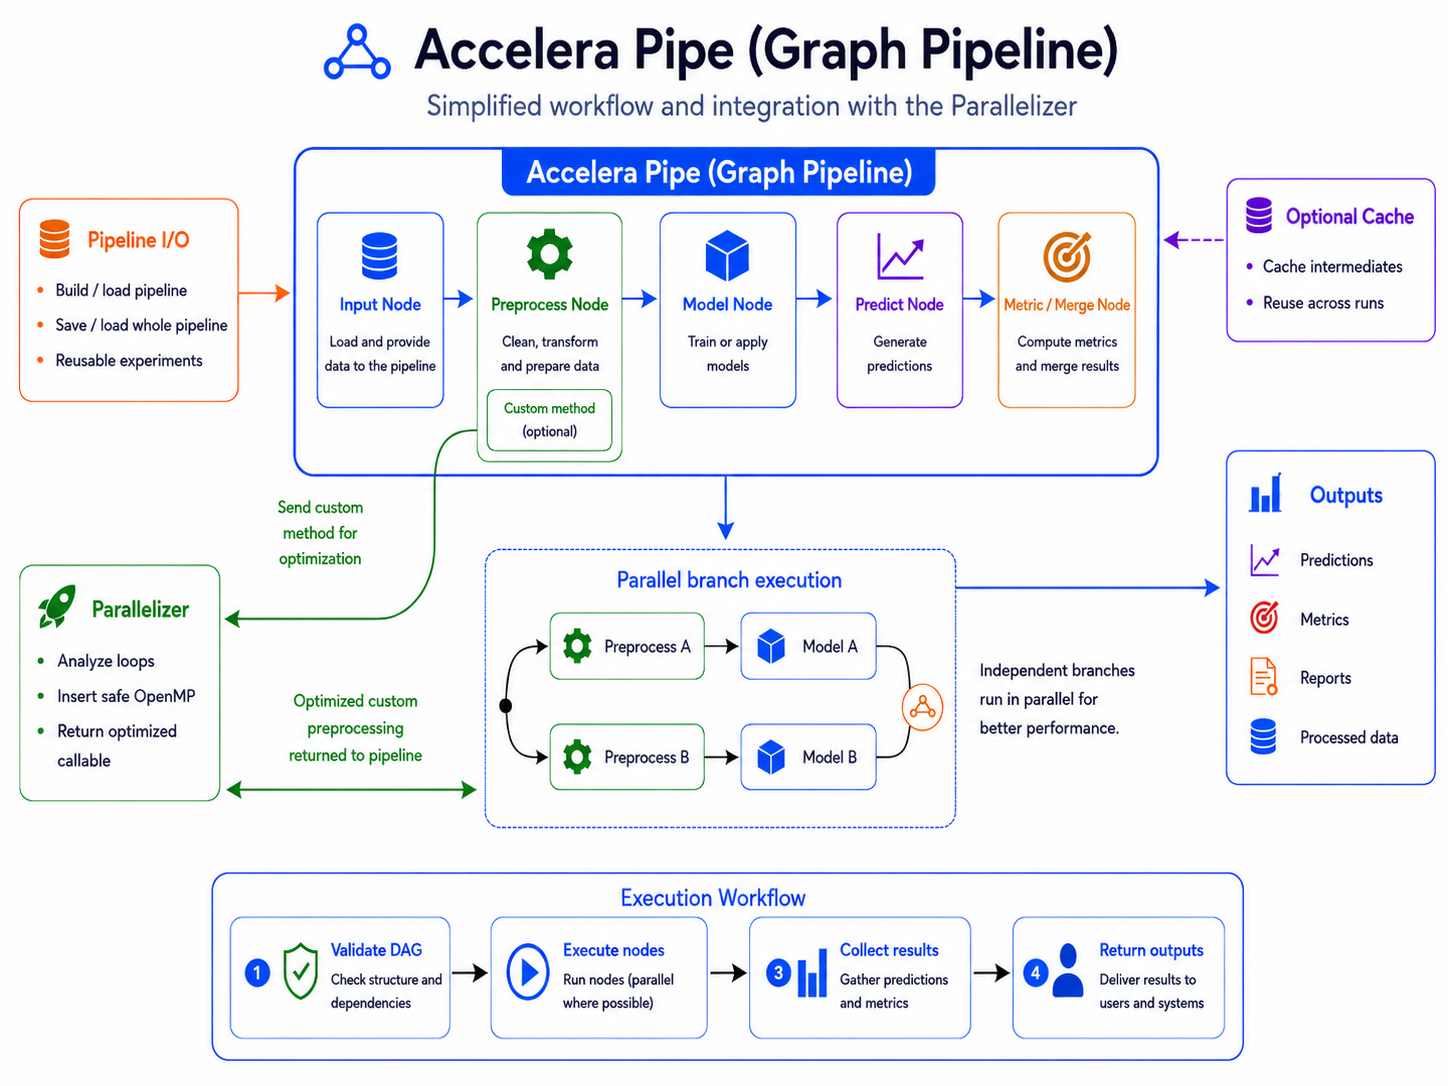
\includegraphics[width=\textwidth,keepaspectratio]{../imgs/accelera_pipe.png}
\caption{Accelera Pipe workflow with custom preprocessing parallelization and pipeline reuse.}
\label{fig:accelera-pipe-workflow}
\end{figure}

As shown in Figure~\ref{fig:accelera-pipe-workflow}, the Python layer provides
the builder interface and communicates with the native C++ graph engine. The
Python layer handles usability, metric wrapping, reports, serialization,
save/load support, and integration with the Code Parallelizer. The C++ layer
stores nodes and edges, validates graph connections, computes the topological
execution order, schedules independent branches, selects the final fitted path,
and manages intermediate memory.

The module also separates training-time execution from inference-time execution.
When a pipeline is called, the native graph executes all required nodes and
returns both the computed predictions or metric results and an
\texttt{ExecutedGraph} object. The \texttt{ExecutedGraph} contains only the
selected fitted execution path and can be reused later for inference. For a new
input \(X_{\text{new}}\), inference can be represented as:
\[
\hat{y} = G^*(X_{\text{new}})
\]
where \(G^*\) is the fitted executed graph selected during training. This
separation is practical because training may require validation data, metrics,
temporary arrays, and candidate branches, while inference should keep only the
fitted transformations and models needed for new data.

Another functional role of Accelera Pipe is transparent optimization of custom
preprocessing logic. When the user provides a custom preprocessing function or a
custom transformer, the pipeline sends it through the Code Parallelizer before
storing it in the graph. If the transformation is safe and supported, loop-heavy
parts can be replaced with a compiled Python-callable C++ implementation. If the
optimization cannot be applied, the original function is kept, so the external
behavior of the pipeline remains unchanged.

\subsection{Module Components}

\begin{table}[H]
\centering
\small
\renewcommand{\arraystretch}{1.15}
\setlength{\tabcolsep}{4pt}
\caption{Main components of the Accelera Pipe module}
\label{tab:accelera-pipe-components}
\begin{tabular}{p{0.30\textwidth}p{0.62\textwidth}}
\toprule
\textbf{Component} & \textbf{Responsibility} \\
\midrule
Pipeline Builder Interface &
Provides the fluent API used to define preprocessing stages, models, prediction
steps, metrics, merge operations, and branches. It translates each user call into
a typed computational node instead of immediately executing it. \\
\midrule
Pipeline State and Persistence Manager &
Owns the native graph object, maps high-level node categories to graph node
types, controls graph execution settings, and provides save/load behavior for
reusable pipeline objects. \\
\midrule
Executed Graph Runtime &
Represents the fitted execution path selected after training. It allows fitted
transformations and models to be reused for inference without keeping validation
data or temporary training branches. \\
\midrule
Metric and Display Wrappers &
Adapt supervised metrics, unsupervised metrics, arrays, figures, dictionaries,
and reports into graph-compatible outputs that can be stored, selected, or
displayed. \\
\midrule
Native Graph Engine &
Stores the pipeline as a DAG, validates node connections, computes execution
order, schedules sequential or parallel execution, manages branch selection, and
controls intermediate-memory lifetime. \\
\midrule
Node Abstraction Layer &
Defines the common behavior of input, preprocessing, model, prediction, merge,
and metric nodes, including source-node relationships, stored data, GPU usage
flags, and selected-path markers. \\
\bottomrule
\end{tabular}
\end{table}

At the Python API level, each builder method creates or configures one graph
operation. A preprocessing node stores a function or transformer together with
execution parameters such as \texttt{execute\_fit} and \texttt{cache}. Model
nodes store estimators, prediction nodes store test data and the prediction
method name, metric nodes store metric wrappers, and merge nodes store the merge
strategy.

\begin{table}[H]
\centering
\small
\renewcommand{\arraystretch}{1.15}
\setlength{\tabcolsep}{4pt}
\caption{Mapping from builder calls to graph node semantics}
\label{tab:accelera-pipe-builder-map}
\begin{tabularx}{\textwidth}{p{0.31\textwidth}p{0.18\textwidth}X}
\toprule
\textbf{Builder method} & \textbf{Node type} & \textbf{Main role} \\
\midrule
\texttt{preprocess(name, func)} &
\texttt{PREPROCESS} &
Transform input data or selected columns. \\
\midrule
\texttt{model(name, model)} &
\texttt{MODEL} &
Fit or apply a machine-learning estimator. \\
\midrule
\texttt{predict(name, test\_data)} &
\texttt{PREDICT} &
Run a model output function such as \texttt{predict}. \\
\midrule
\texttt{metric(name, metric)} &
\texttt{METRIC} &
Evaluate predictions using a supervised or unsupervised metric. \\
\midrule
\texttt{merge(name, strategy)} &
\texttt{MERGE} &
Combine outputs from multiple prediction branches. \\
\midrule
\texttt{branch(name, ...)} &
Multiple nodes &
Create alternative candidate paths in the DAG. \\
\bottomrule
\end{tabularx}
\end{table}

\subsection{Branching and Path Selection}

The native backend uses a graph abstraction rather than a linear pipeline. The
\texttt{Graph} class stores all nodes, tracks whether the graph has already been
compiled, supports cloning, and exposes methods for adding nodes, splitting
branches, executing, clearing, saving, loading, and enabling parallel execution.
The graph computes a topological execution order before running, so each node is
executed only after its source nodes have produced their outputs.

Branching is handled by the native \texttt{split} operation. Each branch is
converted into a chain of graph nodes starting from the current leaf. If the
current leaf node is \(L\), then a branch \(B_i\) can be represented as:
\[
B_i = (L, n_{i1}, n_{i2}, \ldots, n_{ik})
\]
where \(n_{i1}, n_{i2}, \ldots, n_{ik}\) are the operations added to that branch.
This means that all branches start from the same graph point, but each branch can
represent a different candidate workflow, such as a different preprocessing
strategy, model, prediction step, or metric evaluation path.

After branch execution, the graph selects the required path according to the
configured strategy. If \(P = \{B_1, B_2, \ldots, B_m\}\) is the set of candidate
branches and \(M(B_i)\) is the metric value of branch \(B_i\), then a maximization
strategy can be represented as:
\[
B^* = \arg\max_{B_i \in P} M(B_i)
\]
For minimization metrics, the same idea is applied using \(\arg\min\). The
selected branch \(B^*\) is then used to construct the compact executed graph used
later for inference.

A useful optimization in branch construction is duplicate first-node sharing. If
several branches begin with the same first node, the graph creates that first
node once and connects later branch consumers to its output. The sharing
condition can be written as:
\[
n_{11} = n_{21} = \cdots = n_{m1}
\]
where \(n_{i1}\) is the first node of branch \(B_i\). This is safe because all
such branches receive the same original input. The optimization is deliberately
conservative: later repeated nodes are not merged automatically because their
inputs may already differ due to earlier branch operations.

\begin{figure}[H]
\centering
\begin{subfigure}{0.48\linewidth}
    \centering
    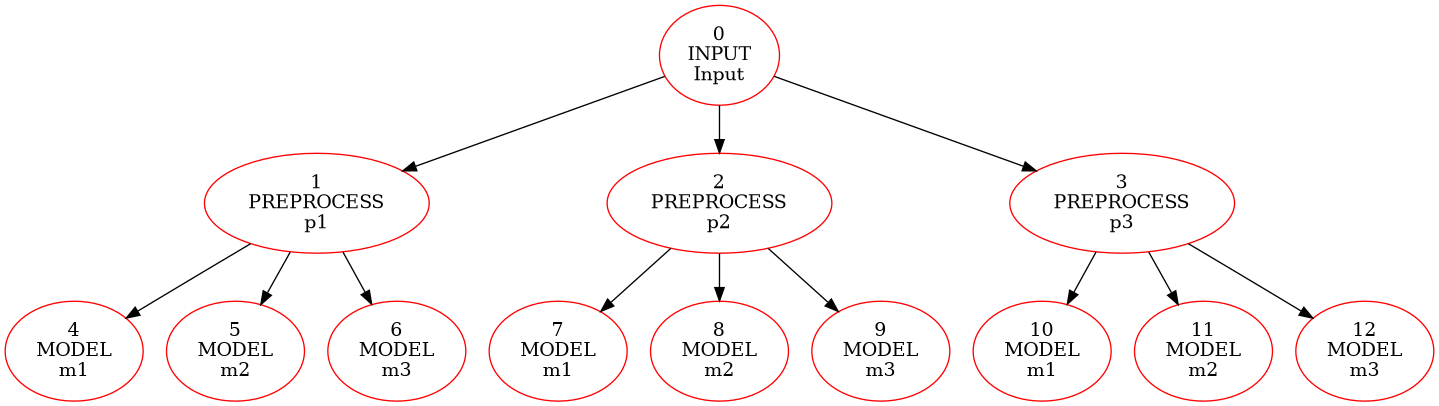
\includegraphics[width=\linewidth]{../imgs/before_sharing.png}
    \caption{Before duplicate first-node sharing}
\end{subfigure}
\hfill
\begin{subfigure}{0.48\linewidth}
    \centering
    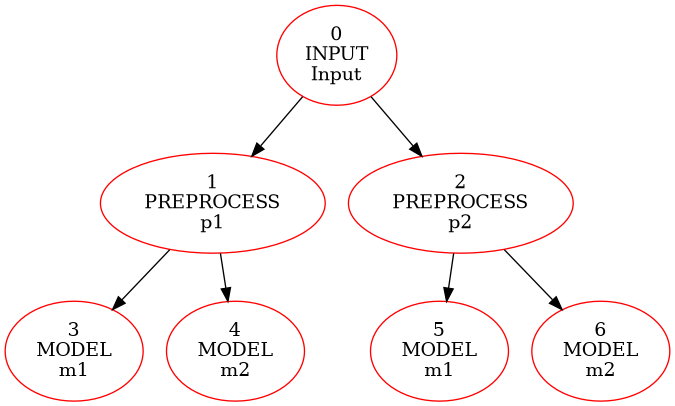
\includegraphics[width=\linewidth]{../imgs/after_sharing.png}
    \caption{After duplicate first-node sharing}
\end{subfigure}
\caption{Branch graph before and after sharing equivalent first branch nodes.}
\label{fig:branch-sharing}
\end{figure}


\subsection{Intermediate Memory Management}

Memory management is an important part of the Accelera Pipe design because
branch-heavy training can create many temporary arrays. If every intermediate
output is kept until the end of execution, the graph may consume unnecessary
memory, especially when several preprocessing and prediction branches are
evaluated together. To reduce this overhead, the backend tracks how many
downstream nodes still need each source output.

For a source node \(S\), the remaining-consumer count is:
\[
C(S) = |\{N \mid S \rightarrow N \text{ and } N \text{ has not executed yet}\}|
\]
This count represents the number of unfinished nodes that still depend on the
output of \(S\). After a downstream consumer finishes, the counter is updated as:
\[
C(S) \leftarrow C(S) - 1
\]
When the counter reaches zero and the source node is safe to clear, the temporary
output can be released:
\[
C(S)=0 \Rightarrow \text{release}(S)
\]
This policy reduces memory pressure without changing the selected path, metric
results, or final predictions. Model and metric nodes are handled more carefully
because they may contain fitted estimators or evaluation state, while temporary
input and preprocessing outputs can often be cleared after their final consumer
has completed.

\begin{lstlisting}[style=algostyle,caption={Consumer-count based intermediate release},label={alg:consumer-release}]
Input: executed node N, remaining consumer table C
Output: graph with unused temporary data released

1:  for each source node S that feeds N do
2:      C[S] = C[S] - 1
3:      if C[S] == 0 and S is releasable then
4:          clear the temporary data stored by S
5:      end if
6:  end for
\end{lstlisting}

Algorithm~\ref{alg:consumer-release} summarizes the release mechanism. The
backend does not randomly clear intermediate values; it clears a source output
only after all of its consumers have finished. This keeps execution correct while
allowing the graph to reuse memory during long or branch-heavy training runs.


\subsection{Parallel Graph Execution}

The graph can run independent nodes in parallel, but a node can start only after
all of its parents have finished. Therefore, parallelism is controlled by both
dependency constraints and hardware-resource constraints. For any node \(N\), the
readiness condition is:
\[
\text{ready}(N) \Longleftrightarrow \forall P \in \text{Parents}(N),\; \text{finished}(P)=\text{true}
\]
This equation means that a node is executable only when every parent node has
already produced its output. If two ready nodes do not depend on each other, they
can be scheduled concurrently.

The backend also limits the number of simultaneously running CPU nodes. If
\(T_{\text{cpu}}\) is the number of available CPU execution slots, then the
number of running CPU nodes must satisfy:
\[
|\text{Running}_{\text{cpu}}| \leq T_{\text{cpu}}
\]
GPU execution is handled more conservatively using a single GPU slot:
\[
|\text{Running}_{\text{gpu}}| \leq 1
\]
This prevents unsafe concurrent GPU access while still allowing CPU-side graph
branches to execute in parallel. The number of CPU threads is based on hardware
concurrency but can be overridden using the
\texttt{ACCELERA\_NUM\_THREADS} environment variable.

\begin{lstlisting}[style=algostyle,caption={Parallel graph execution scheduling},label={alg:parallel-graph-execution}]
Input: topological execution order T
Output: completed graph execution or reported error

1:  Initialize finished and started state for all nodes
2:  Build remaining-consumer counts for intermediate outputs
3:  Create limited CPU worker slots and one GPU execution slot
4:  while unfinished nodes still exist do
5:      for each node N in T do
6:          if N has not started and all parent nodes are finished then
7:              Acquire a CPU slot or the GPU slot depending on N
8:              Mark N as started
9:              Launch N asynchronously
10:             After N finishes:
11:                 Mark N as finished
12:                 Release unused source outputs
13:                 Release the CPU or GPU slot
14:          end if
15:      end for
16:  end while
17:  Wait for all launched tasks
18:  Rethrow any stored node execution error
\end{lstlisting}

Algorithm~\ref{alg:parallel-graph-execution} summarizes the scheduling logic used
by the native backend. The scheduler scans the topological execution order and
starts only nodes whose parents have already finished. Ready nodes are launched
asynchronously, but each node must first acquire the appropriate CPU or GPU
execution slot. After a node finishes, the backend marks it as completed,
releases unused source outputs, and wakes the scheduler so that newly ready
child nodes can start.

Finally, the executed graph must not retain training-only data. After training,
the selected path is cloned, validation data stored inside prediction nodes is
cleared, metric target values are removed, and temporary arrays in the training
graph are released. Both unexecuted and executed graphs can be saved as one
pickle file. During loading, the native graph rebuilds the nodes and reconnects
them using stored source indices. This makes the graph serializable even though
part of the implementation is native C++.


\subsection{Design Constraints}

The Accelera Pipe module has several design constraints that guide how the graph
is constructed, executed, and reused. The first constraint is that the internal
workflow must always remain a valid directed acyclic graph. Since execution
depends on topological ordering, cyclic dependencies are not allowed. For any
edge from node \(u\) to node \(v\), the execution order must satisfy:
\[
u \rightarrow v \Rightarrow \tau(u) < \tau(v)
\]
where \(\tau\) represents the topological order of the graph. This guarantees
that every node is executed only after its required source nodes have already
produced their outputs.

The second constraint is node-type validity. Not every node can be connected to
any other node. For example, a prediction node must follow a model node, a metric
node must follow a prediction or merge node, and a merge node should combine
compatible prediction outputs. These restrictions preserve the semantic meaning
of the pipeline and prevent invalid workflows from reaching the execution stage.

The third constraint is safe memory management. Since branch-heavy workflows can
produce many temporary arrays, the backend must release intermediate data only
when it is no longer needed. For a source node \(S\), the remaining-consumer
count is:
\[
C(S) = |\{N \mid S \rightarrow N \text{ and } N \text{ has not executed yet}\}|
\]
The output of \(S\) can be cleared only when \(C(S)=0\) and the node is safe to
release. This reduces memory pressure without changing the final selected path
or prediction results.

The fourth constraint is parallel execution safety. Independent nodes may run in
parallel, but a node can start only after all of its parent nodes have completed:
\[
\text{ready}(N) \Longleftrightarrow \forall P \in \text{Parents}(N),\;
\text{finished}(P)=\text{true}
\]
This prevents downstream nodes from reading incomplete data. The backend also
uses limited CPU worker slots and a separate GPU slot to avoid unsafe resource
sharing during execution.

Finally, the executed graph must not retain training-only data. After training,
the selected path is cloned into an \texttt{ExecutedGraph}, validation inputs are
removed, metric targets are cleared, and temporary arrays are released. This
keeps the saved inference graph compact and focused only on fitted
transformations and models.


\section{Code Parallelizer Module}
\label{sec:methodology-code-parallelizer}

\subsection{Functional Description}

The Code Parallelizer module transforms supported loop-heavy source code into
optimized C++ code annotated with OpenMP pragmas. It is designed to reduce the
execution time of custom preprocessing functions and standalone code snippets by
identifying loops that can be safely executed in parallel. The module accepts
different input forms: a file path, a source string, a custom Python function, or
a custom transformer instance. Regardless of the input form, the goal is to
normalize the input into a C++ loop-analysis path, detect parallelization
opportunities, and return either parallelized source code or a compiled
Python-callable native function.

For Python input, the module first lowers a restricted Python subset into C++.
This conversion is intentionally limited to predictable language constructs such
as arithmetic expressions, assignments, \texttt{for range(...)} loops,
conditionals, function definitions, array-style indexing, and simple calls. The
resulting C++ code is then analyzed by the same loop extraction path used for
native C/C++ input. This avoids building two separate parallelization pipelines
and ensures that both Python and C++ inputs are judged using the same loop
features and safety checks.

After normalization, the module extracts loop information using native Clang AST
bindings. Each loop is represented by its source code and source-line range. The
Python orchestration layer then computes a fixed loop-feature representation,
uses a classifier service to predict whether the loop is a parallelization
candidate, and validates the decision with rule-based checks. If the loop is
safe, the module injects an OpenMP directive such as
\texttt{\#pragma omp parallel for}. For reduction-like loops, it can also emit a
reduction clause when the reduction variable is valid.

The module has fail-safe behavior. If the input cannot be converted, analyzed,
classified, compiled, or loaded as a native extension, the system falls back to
the original Python function or leaves the code unmodified. This is important
because parallelization is an optimization, not a reason to change the semantic
meaning of the user's program.

\subsection{Module Components}

The Code Parallelizer is decomposed into cooperating components: input
normalization, Python-to-C++ conversion, Clang-based loop extraction, feature
extraction and vectorization, classification with rule-based validation, and
OpenMP/native-extension generation.

\begin{table}[H]
\centering
\fontsize{8.8}{10.5}\selectfont
\setlength{\tabcolsep}{5pt}
\renewcommand{\arraystretch}{0.88}
\caption{Main components of the Code Parallelizer module}
\label{tab:parallelizer-components}
\begin{tabular}{p{0.27\textwidth}p{0.63\textwidth}}
\toprule
\textbf{Component} & \textbf{Responsibility} \\
\midrule
Parallelization Orchestrator &
Receives source strings, file paths, custom functions, and transformer instances.
It coordinates conversion, loop extraction, feature analysis, classification,
pragma insertion, caching, compilation, and fallback behavior. \\
\midrule
Python-to-C++ Converter &
Translates a restricted subset of Python into C++ so Python preprocessing logic
can enter the same static loop-analysis pipeline as native C/C++ code. \\
\midrule
Loop Extraction Engine &
Uses a compiler-style front end to locate loops, record source ranges, and expose
structured loop information for feature extraction and rewriting. \\
\midrule
Feature Extraction and Embedding Generator &
Computes structural, dependency, memory-access, control-flow, arithmetic, and
reduction features, then maps them into a fixed-size numeric representation. \\
\midrule
Classifier and Safety Resolver &
Combines classifier predictions with deterministic safety rules to decide whether
a loop remains sequential, receives a parallel-for pragma, or receives a
reduction pragma. \\
\midrule
OpenMP Rewriter and Native Compiler &
Inserts the selected OpenMP directive, wraps optimized C++ into a Python-callable
extension when needed, builds the native module, and returns the optimized
callable. \\
\midrule
Caching Layer &
Stores processed source and compiled native functions using source-based hashes
to avoid repeated conversion and compilation. \\
\bottomrule
\end{tabular}
\end{table}

Figure~\ref{fig:parallelizer_workflow} summarizes the overall data flow. In
general, supported inputs are normalized into a common C++ loop-analysis path,
while callable Python inputs additionally proceed to PyBind11 extension
generation.

\begin{figure}[H]
\centering
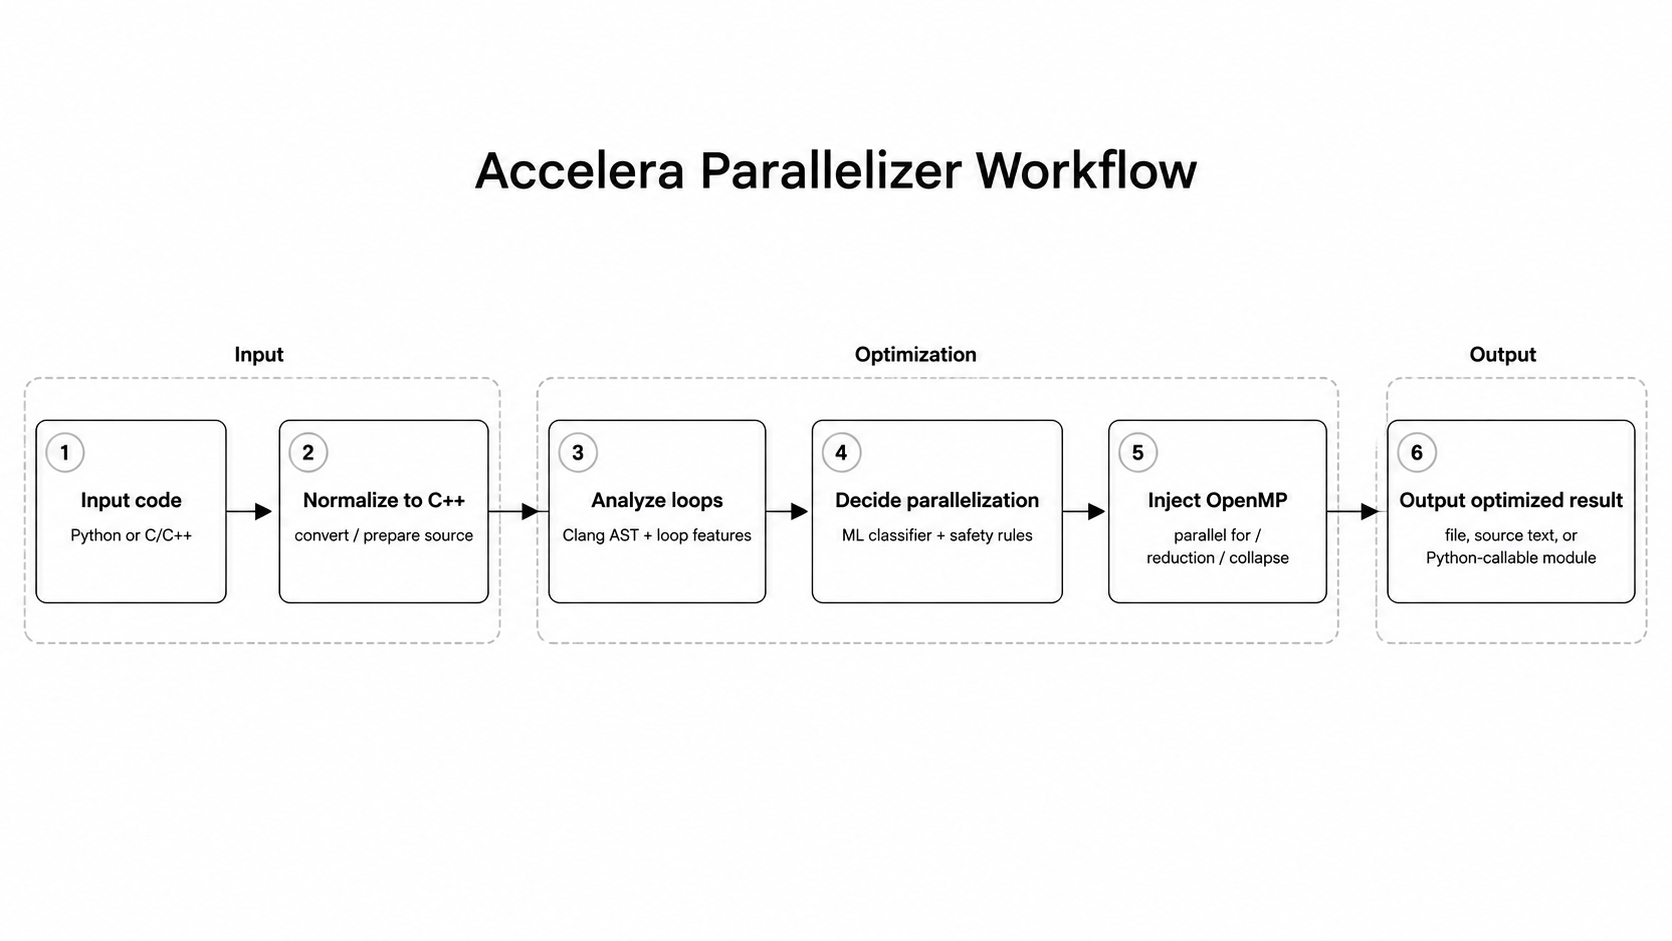
\includegraphics[width=\textwidth,keepaspectratio]{../imgs/p_demo.png}
\caption{Code Parallelizer module workflow}
\label{fig:parallelizer_workflow}
\end{figure}

\subsection{Loop Analysis, Classification, and Conversion}

The feature extraction stage analyzes both code structure and loop behavior,
including reductions, array accesses, dependencies, indirect memory access,
early exits, nesting depth, branches, function calls, arithmetic operations, and
vectorization potential. These indicators are encoded into a 40-dimensional
vector for the classifier, then refined by deterministic safety rules that can
still detect safe cases such as reductions, independent array writes, and nested
loop patterns. The classifier is not treated as the only source of truth; the
rule layer can override the prediction when deterministic evidence proves a safe
or unsafe pattern.

\begin{lstlisting}[style=algostyle,caption={Loop classification and pragma insertion},label={alg:loop-classification}]
Input: source program P
Output: source program P' with safe OpenMP pragmas

1:  if P is Python source then
2:      convert the supported Python subset into C++
3:  end if
4:  Extract for-loops using the Clang AST frontend
5:  for each extracted loop L do
6:      compute structural, memory, dependency, and reduction features
7:      send the 40-feature vector to the classifier service
8:      combine the predicted class with rule-based safety checks
9:      if the resolved class is parallel_for then
10:         insert #pragma omp parallel for
11:     else if the resolved class is reduction then
12:         insert #pragma omp parallel for reduction(...)
13:     else
14:         leave the loop unchanged
15:     end if
16: end for
17: Cache and return the transformed source code
\end{lstlisting}

The Python-to-C++ converter uses Python's \texttt{ast} module and intentionally
supports only a small subset suitable for numeric loops. Unsupported syntax
raises \texttt{ValueError}. Table~\ref{tab:converter} lists the supported
operations.

\begin{table}[H]
\centering
\caption{Supported operations in the Python-to-C++ converter}
\label{tab:converter}
\scriptsize
\begin{tabularx}{\linewidth}{p{0.30\linewidth}X}
\toprule
\textbf{Category} & \textbf{Supported forms and notes} \\
\midrule
Constants and names & \texttt{None}, bool, int, float, string, variables. \\
\midrule
Arithmetic & \texttt{+}, \texttt{-}, \texttt{*}, \texttt{/}, \texttt{\%}, \texttt{**}; power uses \texttt{std::pow}. \\
\midrule
Unary/boolean & unary \texttt{+}, unary \texttt{-}, \texttt{not}, \texttt{and}, \texttt{or}. \\
\midrule
Comparisons & \texttt{==}, \texttt{!=}, \texttt{<}, \texttt{<=}, \texttt{>}, \texttt{>=}; chained comparisons rejected. \\
\midrule
Calls/printing & Ordinary calls and \texttt{print}; keyword arguments are generally unsupported. \\
\midrule
Access & Attribute access and indexing; slices rejected. \\
\midrule
Assignment & Single-target assignment and indexed assignment; multi-target rejected. \\
\midrule
AugAssign & Simple-name \texttt{+=}, \texttt{-=}, \texttt{*=}, \texttt{/=}, and \texttt{\%=}. \\
\midrule
Control flow & \texttt{if}/\texttt{else} and \texttt{return}. \\
\midrule
Loops & \texttt{for i in range(...)} with one, two, or three range arguments. \\
\midrule
Functions & \texttt{def f(...)} as C++ template functions; decorators rejected. \\
\bottomrule
\end{tabularx}
\end{table}

Table~\ref{tab:converter} is intentionally narrow. The converter is not a
general Python compiler; it is a practical bridge for loop-heavy preprocessing
code. By rejecting unsupported constructs early, the Parallelizer avoids
silently generating C++ that changes Python semantics. The supported subset is
enough for examples such as row normalization, scalar reductions, simple
indexing, and range-based nested loops.


\subsection{Integration with Accelera Pipe}

The Code Parallelizer integrates with Accelera Pipe through custom preprocessing
nodes. If \texttt{Pipeline.preprocess()} receives a custom Python function, the
pipeline attempts to optimize it with the Parallelizer before storing it inside
the graph. If it receives a custom transformer object, the transformer instance
can be optimized through its supported preprocessing method. In both cases, the
optimization is best-effort: failed conversion, unsupported syntax, compilation
failure, or module loading failure falls back to the original Python callable.

\begin{figure}[H]
  \centering
  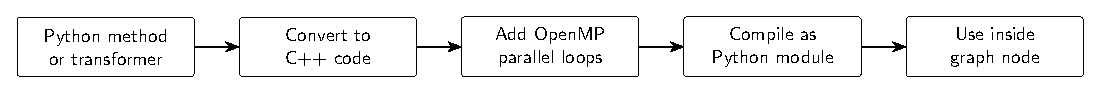
\includegraphics[width=0.94\textwidth]{../imgs/parallelizer_accelera_pipe_flow.pdf}
  \caption{Simplified flow for parallelizing a Python method or transformer and using it inside an Accelera Pipe graph node.}
  \label{fig:integration-flow}
\end{figure}

Figure~\ref{fig:integration-flow} summarizes the integration at a higher level.
The preprocessing callable is converted to C++ when it belongs to the supported
subset, the loop analysis stage adds OpenMP parallelism, and the compiled module
is attached back to the graph node. The graph therefore keeps the same node
structure while replacing eligible Python loops with native execution.

Overall, the Code Parallelizer acts as an optimization layer around user-defined
numeric loops. It does not attempt to parallelize all Python programs. Instead,
it targets the subset where static analysis, feature extraction, classifier
prediction, rule validation, and native compilation can cooperate safely.


\subsection{Design Constraints}

The most important design constraint of the Code Parallelizer is correctness.
OpenMP pragmas can improve performance, but an incorrect pragma can produce
wrong numerical results. Therefore, classifier output is not applied blindly. The
module applies additional safety rules to avoid unsafe transformations when
there are loop-carried dependencies, indirect accesses, early exits, side-effect
function calls, or invalid reduction variables. Inner loops are also skipped
when an outer selected loop already covers their range, preventing nested
duplicate pragma insertion.

The second constraint is the restricted Python subset. Full Python semantics are
too dynamic to translate safely into C++ using a lightweight source converter.
The converter therefore rejects unsupported syntax such as decorators, slicing,
chained comparisons, unsupported operators, non-range loop iterators,
multi-target assignment, complex dynamic dispatch, and unsupported expression
forms. This restriction is a correctness boundary: the system optimizes code
only when it can produce predictable C++.

The third constraint is compiler and platform compatibility. Native callable
optimization depends on a working C++ compiler, Python include paths, PyBind11
headers, NumPy-compatible array wrapping, and platform-specific shared extension
suffixes. The compiler path uses C++17 and adds \texttt{-fopenmp} only when the
parallelized code actually contains OpenMP pragmas. If conversion, compilation,
or module loading fails, the original Python callable is returned.

An earlier generator trial attempted to learn OpenMP pragma generation as a
sequence-to-sequence task. This direction was not selected as the primary
implementation because the available corpus size was too small for robust code
generation and because synthetic examples could introduce distribution bias. A
rule-based and feature-driven design was therefore preferred because it is more
predictable, auditable, and safer for semantic-preserving OpenMP insertion.

\chapter{Experiments and Results}
\label{chap:experiments-and-results}
\section{Controlled Pipeline Comparison}
The main \texttt{accelera\_pipe} experiment compares three implementations of the same four-candidate model-selection task: a manual sklearn loop, sklearn \texttt{Pipeline}, and \texttt{accelera\_pipe}. Each implementation evaluates the same preprocessing alternatives, \texttt{StandardScaler} and \texttt{MinMaxScaler}, and the same model alternatives, \texttt{LogisticRegression} and \texttt{SVC}. Candidate selection is performed on validation accuracy, and final accuracy is reported on the test split only once.

Tables~\ref{tab:latency-scaling} and~\ref{tab:memory-scaling} are the main scalability results. The benchmark starts with 1,000 total samples and grows to 250,000 total samples. Every row keeps the same protocol: 60\% training, 20\% validation, and 20\% test data. Green highlights the fastest runtime for each sample size, while blue highlights the lowest memory usage.

\begin{table}[!htbp]
\centering
\caption{Latency scaling in seconds.}
\label{tab:latency-scaling}
\scriptsize
\begin{tabular}{rrrr}
\toprule
Samples & sklearn & sk Pipe & Accelera \\
\midrule
1{,}000 & 0.06 & \besttime 0.05 & 0.34 \\
5{,}000 & 2.47 & 2.12 & \besttime 2.02 \\
10{,}000 & 2.48 & 2.48 & \besttime 1.79 \\
50{,}000 & 23.96 & 23.25 & \besttime 14.81 \\
100{,}000 & 77.79 & 77.10 & \besttime 67.04 \\
250{,}000 & 803.56 & 803.01 & \besttime 494.64 \\
\bottomrule
\end{tabular}
\end{table}

Table~\ref{tab:latency-scaling} shows the overhead boundary. At 1,000 samples, sklearn Pipeline finishes in 0.05 seconds, while \texttt{accelera\_pipe} takes 0.34 seconds. This is expected because the native graph has setup, node dispatch, and branch-management overhead that cannot be amortized by such a small workload. Starting from 5,000 samples, the pattern changes: \texttt{accelera\_pipe} becomes slightly faster than both sklearn baselines, and the advantage increases as the dataset grows. At 50,000 samples, it reduces runtime from 23.25 seconds for sklearn Pipeline to 14.81 seconds. At 250,000 samples, the reduction is much larger: from 803.01 seconds to 494.64 seconds.

\begin{table}[!htbp]
\centering
\caption{RSS memory delta scaling in MB.}
\label{tab:memory-scaling}
\scriptsize
\begin{tabular}{rrrr}
\toprule
Samples & sklearn & sk Pipe & Accelera \\
\midrule
1{,}000 & 1.62 & \bestmem 0.16 & 19.32 \\
5{,}000 & 3.62 & \bestmem 1.09 & 21.62 \\
10{,}000 & 11.47 & \bestmem 2.19 & 7.25 \\
50{,}000 & 126.95 & \bestmem 9.75 & 209.25 \\
100{,}000 & 139.70 & \bestmem 47.65 & 300.93 \\
250{,}000 & 303.95 & \bestmem 28.52 & 594.86 \\
\bottomrule
\end{tabular}
\end{table}

Table~\ref{tab:memory-scaling} tells the opposite side of the design. sklearn Pipeline has the lowest RSS delta in every row because it runs one candidate pipeline at a time and releases many temporary objects naturally through Python object lifetime. \texttt{accelera\_pipe} keeps graph nodes, branch outputs, and fitted branch state alive during execution, so its RSS delta is higher. This is why the memory optimizations in the methodology are important: consumer-count release, guarded copy removal, duplicate first-node sharing, and training-graph cleanup directly target the gap shown in Table~\ref{tab:memory-scaling}.

\begin{table}[!htbp]
\centering
\caption{Largest controlled comparison run.}
\label{tab:controlled-comparison}
\scriptsize
\begin{tabular}{lrrrr}
\toprule
System & Val. & Test & Time & RSS \\
\midrule
sklearn & 0.9774 & 0.9768 & 803.56 & 303.95 \\
sklearn Pipe & 0.9774 & 0.9768 & 803.01 & 28.52 \\
\texttt{accelera\_pipe} & 0.9774 & 0.9768 & 494.64 & 594.86 \\
\bottomrule
\end{tabular}
\end{table}

Table~\ref{tab:controlled-comparison} isolates the largest run from the scaling experiment because it is the clearest evidence of the latency benefit. The dataset contained 150,000 training samples, 50,000 validation samples, and 50,000 test samples, each with 25 features. All three systems selected an equivalent \texttt{StandardScaler} followed by \texttt{SVC} path and achieved the same test accuracy, 0.9768. This means the runtime improvement is not caused by evaluating a different model, skipping validation, or changing the final test protocol. Under identical candidate selection behavior, \texttt{accelera\_pipe} reduced runtime by 308.91 seconds relative to manual sklearn and 308.36 seconds relative to sklearn Pipeline. The table also makes the current limitation explicit: the faster graph execution pays a memory cost, reaching 594.86 MB RSS delta on this run.

\section{OpenMP Classifier Evaluation}
The Parallelizer classifier is evaluated as a three-class loop classifier. Its output is combined with local rules during pragma generation, but the classifier metrics still describe the quality of the learned loop-feature representation.

The classifier is not expected to be perfect because the final system still applies deterministic checks after prediction. However, Table~\ref{tab:classifier} is useful because it shows whether the learned feature vector can separate the three main loop categories. The \texttt{parallel\_for} class has the highest precision at 0.86, which is important because false positive parallelization can be unsafe. The \texttt{reduction} class has lower support, only 775 examples, but still reaches 0.82 recall. This suggests that the feature extractor captures common scalar-reduction patterns well enough for the classifier to help, while the rule layer remains necessary for safety.

\begin{table}[!htbp]
\centering
\caption{OpenMP classifier test metrics.}
\label{tab:classifier}
\footnotesize
\begin{tabular}{lrrrr}
\toprule
Class & Prec. & Rec. & F1 & Support \\
\midrule
\texttt{none} & 0.82 & 0.85 & 0.84 & 3048 \\
\texttt{parallel\_for} & 0.86 & 0.81 & 0.83 & 2696 \\
\texttt{reduction} & 0.79 & 0.82 & 0.80 & 775 \\
\midrule
Accuracy & \multicolumn{3}{r}{0.83} & 6519 \\
Macro avg. & 0.82 & 0.83 & 0.83 & 6519 \\
Weighted avg. & 0.83 & 0.83 & 0.83 & 6519 \\
\bottomrule
\end{tabular}
\end{table}

The macro and weighted averages are both close to 0.83 F1-score. The macro average treats the three classes equally, so it is sensitive to the smaller \texttt{reduction} class. The weighted average follows the dataset distribution, where \texttt{none} and \texttt{parallel\_for} are more common. The closeness of these two averages indicates that the model is not only performing on the majority classes. In the full Parallelizer, these predictions are used as a first signal, then local rules refine the decision before any OpenMP pragma is emitted.

\section{Parallelizer Hard-File Evaluation}
The hard-file evaluation script parallelizes examples from \texttt{data/hard\_test\_files}, compiles both baseline and generated versions, runs each executable three times, compares outputs, and records timing. Numeric outputs use tolerant comparison because OpenMP reductions can change floating-point accumulation order. Table~\ref{tab:hard-eval} shows the measured results.

\begin{table}[!htbp]
\centering
\caption{Hard-file Parallelizer evaluation.}
\label{tab:hard-eval}
\footnotesize
\begin{tabular}{lrrr}
\toprule
File & Base (ms) & Par. (ms) & Speedup \\
\midrule
\texttt{hard\_eval\_000.cpp} & 1786.28 & 195.47 & 9.138$\times$ \\
\texttt{hard\_eval\_001.cpp} & 63.98 & 31.47 & 2.033$\times$ \\
\texttt{hard\_eval\_002.py} & 42.66 & 7.67 & 5.563$\times$ \\
\bottomrule
\end{tabular}
\end{table}

Table~\ref{tab:hard-eval} evaluates the generated code as executable programs, not only as text. This matters because a pragma can look correct syntactically while still changing output values or failing to compile. The first file obtains the largest speedup, 9.138$\times$, because its workload benefits strongly from parallel loop execution. The second file still improves, but only by 2.033$\times$, which suggests either a smaller loop body, more overhead relative to useful work, or less exploitable parallel work. The third file begins as supported Python, passes through the Python-to-C++ converter, and still reaches 5.563$\times$, which validates the Python conversion path in addition to the C++ pragma insertion path.

The three files were parallelized, compiled, executed, and verified successfully. The report contained 11 extracted loops, 8 gold pragmas, and 8 generated pragmas. Exact pragma matching reached 8 out of 8, and average pragma similarity was 1.0. This means that for these hard examples, the generated pragma text matched the expected OpenMP annotations. The average measured parallelization latency was 231.53 ms, which is small compared with the runtime savings for long-running kernels. Across the three verified files, the average speedup was 5.578$\times$.

\section{Pipeline Integration Benchmark}
The integration experiment uses a custom row-normalization preprocessing function over an input shape of \texttt{(500000, 25)}. The Python implementation contains nested loops that compute the row norm and divide each feature by the norm. The optimized path converts the function to C++, inserts OpenMP, compiles a pybind module, and uses the compiled callable inside \texttt{accelera\_pipe}.

\Needspace{9\baselineskip}
\begin{center}
\captionof{table}{Automatic custom preprocessing acceleration inside \texttt{accelera\_pipe}.}
\label{tab:integration-benchmark}
\footnotesize
\begin{tabularx}{\linewidth}{Xrr}
\toprule
Mode & Samples & Time (s) \\
\midrule
Python custom preprocessing function & 500,000 & 6.83 \\
End-to-end optimized run, first measured process & 500,000 & 5.88 \\
End-to-end optimized run, warmed method and module cache & 500,000 & \besttime 0.08 \\
\bottomrule
\end{tabularx}
\end{center}

The integration benchmark in Table~\ref{tab:integration-benchmark} reports the
direct \texttt{examples/parallel\_accpipe.py} run after normalizing example
execution to the repository root. The pure Python preprocessing function takes 6.83
seconds on 500,000 samples. The first optimized process in the measured
sequence takes 5.88 seconds because process-local setup and cache lookup still
appear in the end-to-end path. The immediate repeated run takes 0.08 seconds
after the Python-method cache and compiled-module cache are both warm. The
example validation confirmed that the optimized output matched the Python
output. This result shows that the integration benefits from two cache layers:
one that avoids repeating Python-to-C++ conversion and OpenMP insertion, and
one that avoids recompiling the pybind extension.

\FloatBarrier

\section{Direct Example Verification Across Operating Systems}
The final verification step runs the same demonstration scripts used by the
project Makefile. These examples are important because they exercise the modules
as a user would run them: graph pipeline execution, automatic preprocessing
optimization, standalone source parallelization, and save/load persistence. The
Linux and Windows measurements should not be compared as hardware-normalized
benchmarks; they are environment verification runs. Their purpose is to confirm
that the examples complete, preserve outputs or accuracy, and expose where
compilation and operating-system overhead appear.

\begin{center}
\captionof{table}{Linux direct example-script verification runs.}
\label{tab:direct-example-runs}
\footnotesize
\begin{tabular}{lrrr}
\toprule
Example & Baseline time (s) & Optimized time (s) & Validation \\
\midrule
\texttt{accpipe\_demo.py} & 2.48 & \besttime 1.79 & same test accuracy, 0.9260 \\
\texttt{parallel\_accpipe.py}, run 1 & 6.83 & \besttime 5.88 & outputs match \\
\texttt{parallel\_accpipe.py}, run 2 & 6.83 & \besttime 0.08 & outputs match \\
\texttt{code\_parallelizer\_demo.py}, run 1 & 5.81 & \besttime 0.014 & outputs match \\
\texttt{code\_parallelizer\_demo.py}, run 2 & 6.05 & \besttime 0.015 & outputs match \\
\texttt{save\_load.py}, run 1 & 1.89 & 2.69 / 2.65 & same accuracy, 0.268 \\
\texttt{save\_load.py}, run 2 & 2.53 & \besttime 2.20 / 2.14 & same accuracy, 0.268 \\
\bottomrule
\end{tabular}
\end{center}

Table~\ref{tab:direct-example-runs} summarizes the Linux examples invoked by
\texttt{examples/Makefile}, but each file was run directly rather than through
Make so that the timing for each demonstration could be read separately.
Cache-sensitive files were repeated. The standalone
\texttt{code\_parallelizer\_demo.py} result measures Python script execution
against the generated OpenMP executable for \texttt{hard\_eval\_002.py}. The C
path also reported about 0.26--0.27 seconds of compilation time outside the
listed executable runtime. The save/load example verifies persistence rather
than pure acceleration: both sklearn and Accelera load persisted state and
produce the same accuracy, while the second Accelera run is slightly faster
than the sklearn baseline.

\par\vspace{0.8em}
\begin{table}[!htbp]
\centering
\caption{Windows direct example correctness and path timing.}
\label{tab:direct-example-runs-windows}

\scriptsize
\renewcommand{\arraystretch}{1.12}
\setlength{\tabcolsep}{3pt}

\begin{tabularx}{\textwidth}{
  >{\raggedright\arraybackslash}p{0.25\textwidth}
  >{\raggedright\arraybackslash}p{0.21\textwidth}
  >{\centering\arraybackslash}p{0.12\textwidth}
  >{\centering\arraybackslash}p{0.15\textwidth}
  >{\raggedright\arraybackslash}X
}
\toprule
Example & Run/cache state & Baseline (s) & Accelera/C path (s) & Validation \\
\midrule

\path{accpipe_demo.py} &
normal &
1.75 / 1.78 &
\besttime 1.03 &
same test accuracy, 0.9260 \\

\path{parallel_accpipe.py} &
isolated cache, run 1 &
6.66 &
\besttime 6.00 &
outputs match \\

\path{parallel_accpipe.py} &
isolated cache, run 2 &
6.58 &
\besttime 0.09 &
outputs match \\

\path{code_parallelizer_demo.py} &
isolated cache, run 1 &
5.59 &
\besttime 1.04 &
outputs match \\

\path{code_parallelizer_demo.py} &
isolated cache, run 2 &
5.61 &
\besttime 1.05 &
outputs match \\

\path{save_load.py} &
normal &
0.57 &
\besttime 0.51 / 0.53 &
same accuracy, 0.268 \\

\bottomrule
\end{tabularx}

\renewcommand{\arraystretch}{1.0}
\normalsize
\end{table}

\begin{table}[!htbp]
\centering
\caption{Windows compilation and process overhead.}
\label{tab:direct-example-runs-windows-overhead}

\scriptsize
\renewcommand{\arraystretch}{1.18}
\setlength{\tabcolsep}{3pt}

\begin{tabularx}{\textwidth}{
  >{\raggedright\arraybackslash}p{0.25\textwidth}
  >{\raggedright\arraybackslash}p{0.21\textwidth}
  >{\centering\arraybackslash}p{0.13\textwidth}
  >{\centering\arraybackslash}p{0.12\textwidth}
  >{\raggedright\arraybackslash}X
}
\toprule
Example & Run/cache state & Compile/link (s) & Wall time (s) & Interpretation \\
\midrule

\path{accpipe_demo.py} &
normal &
-- &
6.53 &
Graph example startup \\

\path{parallel_accpipe.py} &
isolated cache, run 1 &
included &
14.37 &
Cold compile path \\

\path{parallel_accpipe.py} &
isolated cache, run 2 &
cached &
8.33 &
Warm cache path \\

\path{code_parallelizer_demo.py} &
isolated cache, run 1 &
0.87 &
8.74 &
Temporary executable \\

\path{code_parallelizer_demo.py} &
isolated cache, run 2 &
1.04 &
9.00 &
Temporary executable \\

\path{save_load.py} &
normal &
-- &
2.71 &
Persistence example \\

\bottomrule
\end{tabularx}

\renewcommand{\arraystretch}{1.0}
\normalsize
\end{table}

Tables~\ref{tab:direct-example-runs-windows}
and~\ref{tab:direct-example-runs-windows-overhead} report the same Makefile
example set on Windows. The first table keeps the user-visible comparison:
baseline runtime, optimized path runtime, and validation result. The second
table separates compilation and process-level overhead so the timing table can
remain readable. The examples were run one by one in Makefile order. The
cache-sensitive examples were then repeated under an isolated Accelera cache so
that the first run represents cold-cache behavior and the second run represents
warm-cache behavior. The Windows build path also exercises the platform changes
made for the Parallelizer: CMake searches for LLVM/Clang, attempts automatic
installation through Windows package managers when needed, and the runtime
compiler uses the LLVM \texttt{clang++} path without Linux-only flags.

The strongest cache effect appears in \texttt{parallel\_accpipe.py}. The cold
end-to-end Accelera path takes 6.00 seconds because it must extract the Python
function source, convert it to C++, select safe loops, generate OpenMP pragmas,
compile a pybind extension, link it, import it, and attach the compiled
callable to the preprocessing node. The immediate warm-cache run takes
0.09 seconds because the processed-code cache, method cache, and compiled-module
cache avoid repeating those setup stages. This verifies that Windows execution
benefits from the same cache design as Linux, even though the process-level
wall time remains higher.

The Windows \texttt{code\_parallelizer\_demo.py} runs mainly measure end-to-end toolchain latency rather than pure loop speed. 
Each run rebuilds a temporary executable, so the reported wall time includes compilation, process startup, 
OpenMP initialization, dynamic loading, and executable creation. 
The generated program itself reports only about 0.024--0.025 seconds for the timed main-body work, 
while Linux has lower launch and linking overhead, making its runtime closer to the measured kernel work.

% -----------------------------------------------------------------------------
\chapter{Conclusion}
\label{chap:conclusion}
The two examined modules address complementary bottlenecks. \texttt{accelera\_pipe} improves workflow-level execution by representing candidate pipelines as a graph, running branches in parallel, selecting paths through metrics, reusing executed graphs for inference, and reducing temporary data retention. The Parallelizer improves loop-level execution by converting supported Python code to C++, extracting loops, classifying OpenMP opportunities, and compiling supported custom preprocessing functions into native Python-callable modules.

The current results show that the graph executor can match sklearn accuracy while reducing large benchmark latency, and that the Parallelizer can produce substantial speedups for both standalone hard loop files and integrated preprocessing kernels. Future work should expand the literature review, broaden the Python-to-C++ subset, improve memory usage during branch-heavy searches, and refine compile-cache policy for interactive workflows.

\begin{thebibliography}{9}

\bibitem{pedregosa2011scikit}
F. Pedregosa, G. Varoquaux, A. Gramfort, V. Michel, B. Thirion,
O. Grisel, M. Blondel, P. Prettenhofer, R. Weiss, V. Dubourg,
J. Vanderplas, A. Passos, D. Cournapeau, M. Brucher, M. Perrot,
and E. Duchesnay,
``Scikit-learn: Machine Learning in Python,''
\textit{Journal of Machine Learning Research}, vol. 12, pp. 2825--2830, 2011.

\bibitem{ompar2024}
T. Kadosh, N. Hasabnis, P. Soundararajan, V. A. Vo, M. Capota,
N. Ahmed, Y. Pinter, and G. Oren,
``OMPar: Automatic Parallelization with AI-Driven Source-to-Source Compilation,''
arXiv preprint arXiv:2409.14771, 2024.

\end{thebibliography}


\end{document}
